\documentclass[]{article}
\usepackage{lmodern}
\usepackage{amssymb,amsmath}
\usepackage{ifxetex,ifluatex}
\usepackage{fixltx2e} % provides \textsubscript
\ifnum 0\ifxetex 1\fi\ifluatex 1\fi=0 % if pdftex
  \usepackage[T1]{fontenc}
  \usepackage[utf8]{inputenc}
\else % if luatex or xelatex
  \ifxetex
    \usepackage{mathspec}
  \else
    \usepackage{fontspec}
  \fi
  \defaultfontfeatures{Ligatures=TeX,Scale=MatchLowercase}
\fi
% use upquote if available, for straight quotes in verbatim environments
\IfFileExists{upquote.sty}{\usepackage{upquote}}{}
% use microtype if available
\IfFileExists{microtype.sty}{%
\usepackage{microtype}
\UseMicrotypeSet[protrusion]{basicmath} % disable protrusion for tt fonts
}{}
\usepackage[margin=1in]{geometry}
\usepackage{hyperref}
\hypersetup{unicode=true,
            pdftitle={Usando clustering para identificar cursos no Prouni},
            pdfauthor={Pedro Cavalcante},
            pdfborder={0 0 0},
            breaklinks=true}
\urlstyle{same}  % don't use monospace font for urls
\usepackage{color}
\usepackage{fancyvrb}
\newcommand{\VerbBar}{|}
\newcommand{\VERB}{\Verb[commandchars=\\\{\}]}
\DefineVerbatimEnvironment{Highlighting}{Verbatim}{commandchars=\\\{\}}
% Add ',fontsize=\small' for more characters per line
\usepackage{framed}
\definecolor{shadecolor}{RGB}{248,248,248}
\newenvironment{Shaded}{\begin{snugshade}}{\end{snugshade}}
\newcommand{\KeywordTok}[1]{\textcolor[rgb]{0.13,0.29,0.53}{\textbf{#1}}}
\newcommand{\DataTypeTok}[1]{\textcolor[rgb]{0.13,0.29,0.53}{#1}}
\newcommand{\DecValTok}[1]{\textcolor[rgb]{0.00,0.00,0.81}{#1}}
\newcommand{\BaseNTok}[1]{\textcolor[rgb]{0.00,0.00,0.81}{#1}}
\newcommand{\FloatTok}[1]{\textcolor[rgb]{0.00,0.00,0.81}{#1}}
\newcommand{\ConstantTok}[1]{\textcolor[rgb]{0.00,0.00,0.00}{#1}}
\newcommand{\CharTok}[1]{\textcolor[rgb]{0.31,0.60,0.02}{#1}}
\newcommand{\SpecialCharTok}[1]{\textcolor[rgb]{0.00,0.00,0.00}{#1}}
\newcommand{\StringTok}[1]{\textcolor[rgb]{0.31,0.60,0.02}{#1}}
\newcommand{\VerbatimStringTok}[1]{\textcolor[rgb]{0.31,0.60,0.02}{#1}}
\newcommand{\SpecialStringTok}[1]{\textcolor[rgb]{0.31,0.60,0.02}{#1}}
\newcommand{\ImportTok}[1]{#1}
\newcommand{\CommentTok}[1]{\textcolor[rgb]{0.56,0.35,0.01}{\textit{#1}}}
\newcommand{\DocumentationTok}[1]{\textcolor[rgb]{0.56,0.35,0.01}{\textbf{\textit{#1}}}}
\newcommand{\AnnotationTok}[1]{\textcolor[rgb]{0.56,0.35,0.01}{\textbf{\textit{#1}}}}
\newcommand{\CommentVarTok}[1]{\textcolor[rgb]{0.56,0.35,0.01}{\textbf{\textit{#1}}}}
\newcommand{\OtherTok}[1]{\textcolor[rgb]{0.56,0.35,0.01}{#1}}
\newcommand{\FunctionTok}[1]{\textcolor[rgb]{0.00,0.00,0.00}{#1}}
\newcommand{\VariableTok}[1]{\textcolor[rgb]{0.00,0.00,0.00}{#1}}
\newcommand{\ControlFlowTok}[1]{\textcolor[rgb]{0.13,0.29,0.53}{\textbf{#1}}}
\newcommand{\OperatorTok}[1]{\textcolor[rgb]{0.81,0.36,0.00}{\textbf{#1}}}
\newcommand{\BuiltInTok}[1]{#1}
\newcommand{\ExtensionTok}[1]{#1}
\newcommand{\PreprocessorTok}[1]{\textcolor[rgb]{0.56,0.35,0.01}{\textit{#1}}}
\newcommand{\AttributeTok}[1]{\textcolor[rgb]{0.77,0.63,0.00}{#1}}
\newcommand{\RegionMarkerTok}[1]{#1}
\newcommand{\InformationTok}[1]{\textcolor[rgb]{0.56,0.35,0.01}{\textbf{\textit{#1}}}}
\newcommand{\WarningTok}[1]{\textcolor[rgb]{0.56,0.35,0.01}{\textbf{\textit{#1}}}}
\newcommand{\AlertTok}[1]{\textcolor[rgb]{0.94,0.16,0.16}{#1}}
\newcommand{\ErrorTok}[1]{\textcolor[rgb]{0.64,0.00,0.00}{\textbf{#1}}}
\newcommand{\NormalTok}[1]{#1}
\usepackage{graphicx,grffile}
\makeatletter
\def\maxwidth{\ifdim\Gin@nat@width>\linewidth\linewidth\else\Gin@nat@width\fi}
\def\maxheight{\ifdim\Gin@nat@height>\textheight\textheight\else\Gin@nat@height\fi}
\makeatother
% Scale images if necessary, so that they will not overflow the page
% margins by default, and it is still possible to overwrite the defaults
% using explicit options in \includegraphics[width, height, ...]{}
\setkeys{Gin}{width=\maxwidth,height=\maxheight,keepaspectratio}
\IfFileExists{parskip.sty}{%
\usepackage{parskip}
}{% else
\setlength{\parindent}{0pt}
\setlength{\parskip}{6pt plus 2pt minus 1pt}
}
\setlength{\emergencystretch}{3em}  % prevent overfull lines
\providecommand{\tightlist}{%
  \setlength{\itemsep}{0pt}\setlength{\parskip}{0pt}}
\setcounter{secnumdepth}{0}
% Redefines (sub)paragraphs to behave more like sections
\ifx\paragraph\undefined\else
\let\oldparagraph\paragraph
\renewcommand{\paragraph}[1]{\oldparagraph{#1}\mbox{}}
\fi
\ifx\subparagraph\undefined\else
\let\oldsubparagraph\subparagraph
\renewcommand{\subparagraph}[1]{\oldsubparagraph{#1}\mbox{}}
\fi

%%% Use protect on footnotes to avoid problems with footnotes in titles
\let\rmarkdownfootnote\footnote%
\def\footnote{\protect\rmarkdownfootnote}

%%% Change title format to be more compact
\usepackage{titling}

% Create subtitle command for use in maketitle
\newcommand{\subtitle}[1]{
  \posttitle{
    \begin{center}\large#1\end{center}
    }
}

\setlength{\droptitle}{-2em}

  \title{Usando clustering para identificar cursos no Prouni}
    \pretitle{\vspace{\droptitle}\centering\huge}
  \posttitle{\par}
    \author{Pedro Cavalcante}
    \preauthor{\centering\large\emph}
  \postauthor{\par}
      \predate{\centering\large\emph}
  \postdate{\par}
    \date{2018-08-09}


\begin{document}
\maketitle

Você provavelmente conhece alguém que se formou no ensino médio e foi
fazer um infame \emph{cursinho} pensando em uma aprovação numa graduação
em Medicina. Pois é esperado, são cursos estranhamente competitivos e
com as - de longe - maiores notas de corte. Por serem tão anômalos,
podem ser um exercício interessante de classificação.

Vou expor brevemente a matemática por trás do processo de
\emph{Clustering k-means}, alguns problemas que surgem na hora de
aplicar o algoritimo e aplica-lo em uma questão interessante de economia
da educação, \emph{carrer choice}.

\subsection{O que é clustering?}\label{o-que-e-clustering}

Clustering é uma classe de algoritimos não-supervisionados para
classificação de observações. Existem vários tipos, cores e tamanho de
técnicas de clustering, mas essa bonita variedade vai ficar para outro
dia porque o foco de hoje é a abordagem de distância centrada.

\begin{figure}
\centering
\includegraphics{https://i.imgur.com/S65Sk9c.jpg}
\caption{``Agrupamento de observações''}
\end{figure}

A visualização é razoavelmente clara, clusters são literalmente
agrupamentos. Com base em alguns critérios dependentes do algoritimo a
ser utilizado, você classifica uma observação em um \emph{ou} outro
agrupamento (exceto nos modelos \emph{fuzzy}, mas isso fica para outro
dia).

\subsection{Clustering k-means como um problema de
otimização}\label{clustering-k-means-como-um-problema-de-otimizacao}

Um problema de otimização irrestrita tem, a grosso modo, dois
\emph{features}. A \emph{função objetivo} a ser maximizada ou minimizada
e o \emph{instrumento} com o qual atingir tal objetivo. Aqueles
familiarizados com o canônico método de estimação por Mínimos Quadrados
Ordinários vão reconhecer alguma semelheança.

K-means, ao invés de minimizar quadrado dos resíduos, minimiza a soma do
quadrado da distância dentro do cluster (WCSS, em inglês). Nossos
instrumentos são \(k\), o número de agrupamentos e \(S_i\), os conjuntos
que dão qual elemento está em qual agrupamento. Podem parecer
instrumentos redundantes à primeira vista. Pense que para um mesmo
número de agrupamentos, é possível ter combinações de conjuntos com
WCSSs diferentes.

Algumas definições antes. \(k\) é o número de clusters, \(S_i\) é
conjunto de elementos do i-ésimo cluster, \(\mu_i\) é a média do i-ésimo
cluster.

\[ \text{arg min}_S \sum_{i=1}^k \sum_{x_j \in S_i} || x_j - \mu_i ||^2 \]

O leitor atento percebeu que \(k\) não aparece aqui como um instrumento
do problema, mas sim como um parâmetro dado. Bem, aí está uma das
peculiaridades de k-means, \emph{nós escolhemos o k}. É uma tarefa que
tem um pouco de ciência e muita arte, vou me aprofundar um pouco nela
mais à frente.

\subsection{Os dados}\label{os-dados}

A amostra que temos é do ProUni de 2017 e conta com algo em torno de 32
mil observações. Já tive o trabalho de limpar a base para vossa
apreciação e vou deixa-la disponível
\href{https://github.com/danmrc/azul/tree/master/content/post/ProUni}{aqui}
e o código que contém tudo
\href{https://github.com/danmrc/azul/blob/master/content/post/ProUni/prouni_cluster.R}{aqui}.
Vamos primeiro explorar nossa amostra com a ajuda do \texttt{ggplot2}.

\includegraphics{2018-08-09-prouni_files/figure-latex/imagem1-1.pdf}

\begin{figure}
\centering
\includegraphics{https://i.imgur.com/i5yfR5V.png}
\caption{Mapa de densidade de notas de corte, mensalidades. Observações
em azul mais claro são de Medicina.}
\end{figure}

\begin{verbatim}
## Warning: Removed 365 rows containing non-finite values (stat_bin).
\end{verbatim}

\begin{verbatim}
## Warning: Removed 365 rows containing non-finite values (stat_density).
\end{verbatim}

\includegraphics{2018-08-09-prouni_files/figure-latex/imagem2-1.pdf}
\includegraphics{https://i.imgur.com/twn7b7n.png}

\includegraphics{2018-08-09-prouni_files/figure-latex/imagem3-1.pdf}

\includegraphics{https://i.imgur.com/14R87DN.png} Os próximos dois
gráficos tem códigos análogos aos dois anteriores e estão disponíveis no
script.

Aqui observamos três coisas muito interessantes. A primeira é que notas
de corte seguem muito bem uma distribuição normal \emph{exceto} pela
regra que impõe nota de corte mínima de 450 no ProUni e Sisu. É o tipo
de coisa em que seria legal aplicar um
\href{https://eml.berkeley.edu/~jmccrary/mccrary2006_DCdensity.pdf}{Teste
de Densidade de McCrary (2006)}. Depois, que Medicina tem um padrão de
distribuição de notas bem diferente do resto.

\begin{figure}
\centering
\includegraphics{https://i.imgur.com/sipwjrG.png}
\caption{Histograma das notas de corte}
\end{figure}

\begin{figure}
\centering
\includegraphics{https://i.imgur.com/VjfJH7K.png}
\caption{Histograma das notas de corte diferenciando Medicina}
\end{figure}

\subsection{Como escolher k?}\label{como-escolher-k}

Essa é a pergunta de um milhão de dólares, honestamente. Eu encontrei
dois principais métodos, um é computacionalmente exigente e preciso, o
outro é computacionalmente simples e depende mais de interpretação.

A primeira e mais complicada é a \emph{Gap Statistic}
(\href{https://statweb.stanford.edu/~gwalther/gap}{Tbishirani, Walther e
Hastie, 2001}). O método envolve algumas computações com bootstrap,
então exige uma máquina preparada. Só consegui rodar usando um servidor,
então evite esse método se tiver um computador normal (ou até mesmo um
pessoal de alta qualidade). Em qualquer caso, a implementação desse
método é a função \texttt{cluster::clusGap}.

O segundo método é o do ``Cotovelo''. Não é muito sofisticado, mas é
potente. Plotamos o WCSS como uma função de \(k\) e procuramos por uma
inflexão na curva. Onde ela tiver um ``cotovelo'', é provavelmente o
\(k\) mais adequado. A função a seguir implementa o gráfico:

\begin{Shaded}
\begin{Highlighting}[]
\NormalTok{#### Limpar valores lógicos e de texto antes}
\NormalTok{final}\OperatorTok{$}\NormalTok{label <-}\StringTok{ }\OtherTok{NULL}
\NormalTok{final}\OperatorTok{$}\NormalTok{completo <-}\StringTok{ }\OtherTok{NULL}

\NormalTok{#### Definir função para método do Cotovelo}

\NormalTok{wssplot <-}\StringTok{ }\ControlFlowTok{function}\NormalTok{(data, }\DataTypeTok{nc=}\DecValTok{15}\NormalTok{, }\DataTypeTok{seed=}\DecValTok{1234}\NormalTok{)\{}
\NormalTok{  wss <-}\StringTok{ }\NormalTok{(}\KeywordTok{nrow}\NormalTok{(data)}\OperatorTok{-}\DecValTok{1}\NormalTok{)}\OperatorTok{*}\KeywordTok{sum}\NormalTok{(}\KeywordTok{apply}\NormalTok{(data,}\DecValTok{2}\NormalTok{,var))}
  \ControlFlowTok{for}\NormalTok{ (i }\ControlFlowTok{in} \DecValTok{2}\OperatorTok{:}\NormalTok{nc)\{}
    \KeywordTok{set.seed}\NormalTok{(seed)}
\NormalTok{    wss[i] <-}\StringTok{ }\KeywordTok{sum}\NormalTok{(}\KeywordTok{kmeans}\NormalTok{(data, }\DataTypeTok{centers=}\NormalTok{i)}\OperatorTok{$}\NormalTok{withinss)\}}
  
  \KeywordTok{plot}\NormalTok{(}\DecValTok{1}\OperatorTok{:}\NormalTok{nc, wss, }\DataTypeTok{type=}\StringTok{"b"}\NormalTok{, }\DataTypeTok{xlab=}\StringTok{"Number of Clusters"}\NormalTok{,}
       \DataTypeTok{ylab=}\StringTok{"Within groups sum of squares"}\NormalTok{)\}}

\KeywordTok{wssplot}\NormalTok{(final, }
          \DataTypeTok{nc =} \DecValTok{6}\NormalTok{) }
\end{Highlighting}
\end{Shaded}

\includegraphics{2018-08-09-prouni_files/figure-latex/cotovelo-1.pdf}

\begin{figure}
\centering
\includegraphics{https://i.imgur.com/nEBZbL3.png}
\caption{Método do Cotovelo}
\end{figure}

Agora que escolhemos o número 3, podemos finalmente ver se o modelo
classifica bem cursos de medicina.

\subsection{Os finalmentes, rodando o modelo e
resultados}\label{os-finalmentes-rodando-o-modelo-e-resultados}

Tendo 3 como o número mágico, podemos finalmente rodar o modelo.
\texttt{kmeans} é um comando nativo do R, mas visualização pode ser
melhor - afinal, é interessante \emph{ver} os agrupamentos. Para isso,
vamos usar \texttt{cluster::clusplot}:

\begin{Shaded}
\begin{Highlighting}[]
\NormalTok{analise_kmeans <-}\StringTok{ }\KeywordTok{kmeans}\NormalTok{(final, }
                          \DataTypeTok{centers =} \DecValTok{3}\NormalTok{)}

\NormalTok{##### Agora visualize os resultados}

\KeywordTok{clusplot}\NormalTok{(final, analise_kmeans}\OperatorTok{$}\NormalTok{cluster,}
                        \DataTypeTok{main=}\StringTok{'Procurando por 3 agrupamentos no ProUni'}\NormalTok{,}
                            \DataTypeTok{color=}\OtherTok{TRUE}\NormalTok{,}
                              \DataTypeTok{shade=}\OtherTok{TRUE}\NormalTok{,}
                                \DataTypeTok{lines=}\DecValTok{0}\NormalTok{)}
\end{Highlighting}
\end{Shaded}

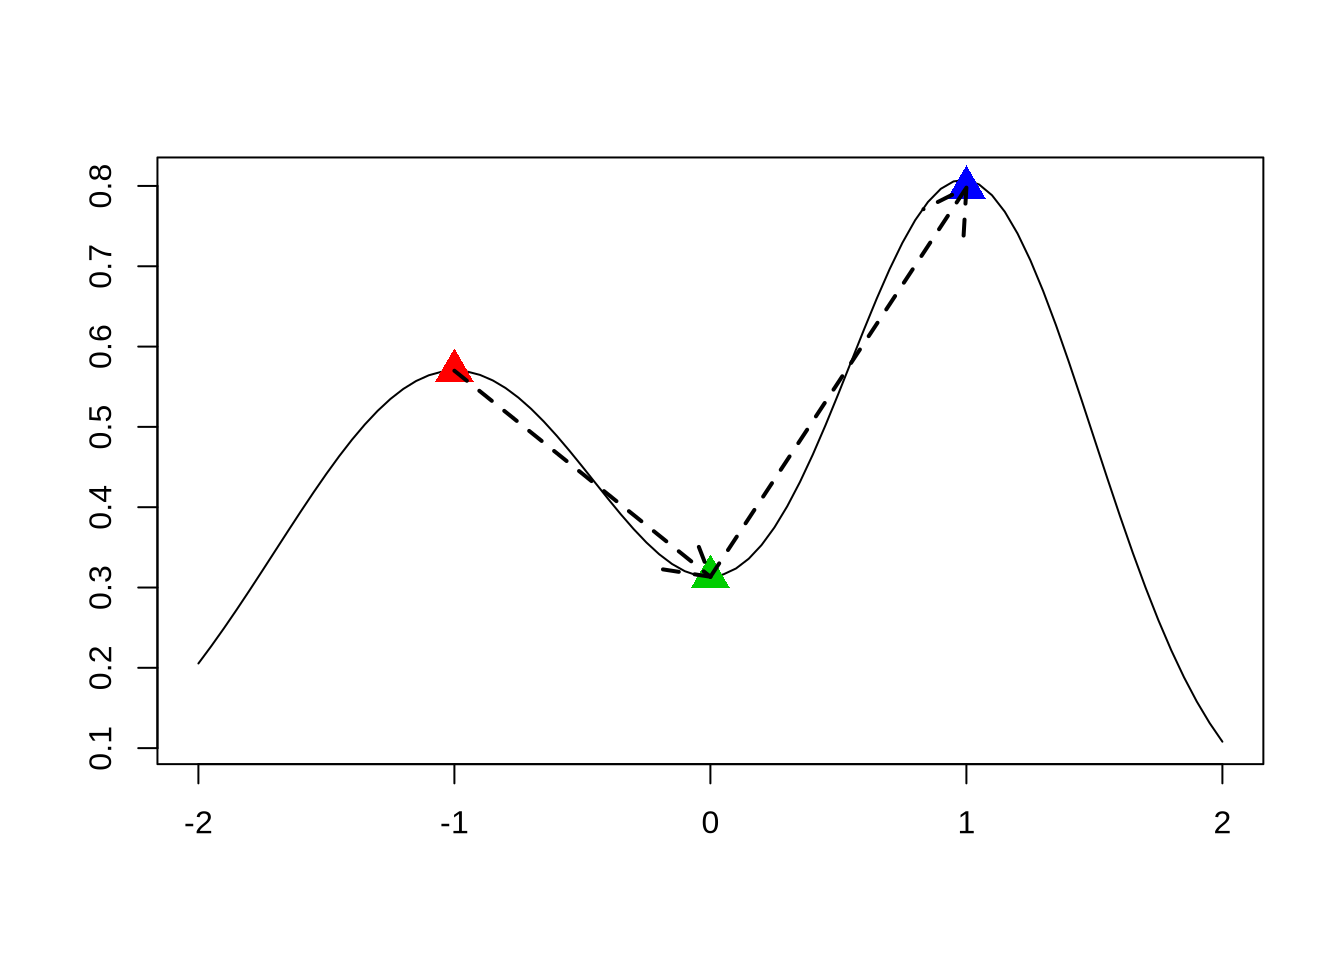
\includegraphics{2018-08-09-prouni_files/figure-latex/unnamed-chunk-1-1.pdf}
\includegraphics{https://i.imgur.com/DO5ZdtC.png}

Se o leitor fizer o exercício de replicar esse post, vai poder ver que o
algoritimo identificou todos os 122 cursos de medicina da amostra e
inseriu por engano no mesmo cluster 44 cursos que não são de medicina.

A performance é aceitável?


\end{document}
